%----------------------------------------------------------------------------------------
%    PACKAGES AND THEMES
%----------------------------------------------------------------------------------------

\documentclass[aspectratio=169,xcolor=dvipsnames]{beamer}
\usetheme{SimplePlus}

\usepackage{hyperref}
\usepackage{graphicx} % Allows including images
\usepackage{booktabs} % Allows the use of \toprule, \midrule and \bottomrule in tables
\usepackage{bbm}
\usepackage[authoryear,round]{natbib}
\usepackage{tikz}
\usetikzlibrary{arrows.meta, positioning}
\usepackage{amsmath}

\DeclareMathOperator*{\argmin}{arg\,min}
\DeclareMathOperator*{\argmax}{arg\,max}

%----------------------------------------------------------------------------------------
%    TITLE PAGE
%----------------------------------------------------------------------------------------

\title{SimplePlus Beamer Theme}
\subtitle{Subtitle}

\author{Zhenxiao Chen}

\institute
{
    Department of Economics \\
    University of Pennsylvania % Your institution for the title page
}
\date{\today} % Date, can be changed to a custom date

%----------------------------------------------------------------------------------------
%    PRESENTATION SLIDES
%----------------------------------------------------------------------------------------

\begin{document}

\begin{frame}
    % Print the title page as the first slide
    \titlepage
\end{frame}

\begin{frame}{Overview}
    % Throughout your presentation, if you choose to use \section{} and \subsection{} commands, these will automatically be printed on this slide as an overview of your presentation
    \tableofcontents
\end{frame}

%------------------------------------------------
\section{Problem Setup}
%------------------------------------------------
\begin{frame}{Preview}
    \begin{itemize}
        \item A simple statistical treatment allocation problem 
            \[
                \max_{\phi \in \Phi}
                \mathbb{E}\left[
                Y(1)\phi(X) + Y(0)(1- \phi(X))
                \right]
            \]
        \item The first-best:
            \[
                \phi^*(x) = \mathbbm{1}\{h_0(x) \geq 0\}, \quad h_0(x) := \mathbb{E}[Y(1) -Y(0) \mid X=x] = \text{CATE}(x)
            \]
        \item Policy learning: What is the best policy under a (un)constrained policy class
            \[
            \hat{\phi}(x) = \mathbbm{1}\{x\in G^*\} \in \argmin_{G \in \mathcal{G}} \frac{1}{n}\sum_{i=1}^n\left(\frac{Y_i D_i}{e(X_i)} - \frac{Y_i(1-D_i)}{1-e(X_i)}\right)\mathbbm{1}\{X_i \in G\}
            \]

        \item \textcolor{blue}{Inference on optimal policy value:} Draw inference on the value of the first-best rule
            \[
            W(h_0) = \int_\mathcal{X}\mathbbm{1}\{h_0(x) \geq 0\}h_0(x)f(x)dx, \quad V(h_0) = \int_\mathcal{X}\mathbbm{1}\{h_0(x) \geq 0\}v_0(x)f(x)dx
            \]
    \end{itemize}
\end{frame}

\begin{frame}{Preview}
    \begin{itemize}
        \item In \citet*{chen2025inference}, we studied an upper-contour integral functional 
            \[
                \Phi(h_0) = \int_\mathcal{X}\mathbbm{1}\{h_0(x) \geq 0\}\phi(h_0(x),x)f(x)dx = \int_{\{h_0(x) \geq 0\}}\phi(h_0(x),x)f(x)dx,
            \]
            where the boundary $\{h_0(x) = 0\}$ is smooth and a well-defined submanifold.
            \begin{itemize}
                \item[-] $\Phi(h_0) = W(h_0)$ when $\phi(h_0(x),x) = h_0(x)$
                \item[-] $\Phi(h_0) = V(h_0)$ when $\phi(h_0(x),x) = v_0(x)$
            \end{itemize}
    \end{itemize}
\end{frame}

\begin{frame}{Preview}
    \begin{itemize}
        \item Contribution: Compute the pathwise derivative via the \textcolor{blue}{Generalized Leibniz Rule}
            \begin{align*}
                \frac{d \Phi(h_0 + t(h-h_0))}{dt}\Bigg|_{t=0}   &= \int \mathbbm{1}\{h_0(x) \geq 0\}\partial_1\phi(h_0(x), x)(h(x) - h_0(x))f(x)dx\\
                &+ \int_{\textcolor{blue}{\{x\in \mathcal{X} :h_0(x) = 0\}}}\frac{h(x) - h_0(x)}{||\nabla_xh_0(x)||}\phi(h_0(x),x)f(x)\textcolor{blue}{d\mathcal{H}^{d-1}(x)}
            \end{align*}
            \begin{itemize}
                \item[-] Pathwise derivative captures the first-order impact of estimating $h_0$ for $W(h_0)$
                \item[-] The first-order impact is two-fold: one comes from perturbing the integrand; the other comes from perturbing the boundary $\{x:h_0(x)=0\}$
                \item[-] \textcolor{blue}{The second term is nonstandard:} does not have a well-defined Riesz representer in $L_2(P)$ $\Rightarrow$ plug-in estimator does not converge in parametric rate
            \end{itemize}
    \end{itemize}
\end{frame}

\begin{frame}{Preview}
    \begin{itemize}
        \item Contribution: Inference for regular and irregular optimal policy values
                \[
                \frac{\sqrt{n}(\Phi(\hat{h}) - \Phi(h_0))}{V_K^{1/2}} \xrightarrow[]{d}\mathcal{N}(0,1), \quad V_K = \mathbb{E}[(\nu_K^*(X_i)\epsilon_i)^2]
                \] 
                \begin{itemize}
                    \item[-] Consider a linear sieve semiparametric plug-in estimator  $\Phi(\hat{h})$ for $\Phi(h_0)$
                    \item[-] Approximate $L_2(P)$ using a sequence of linear sieve spaces, where sieve Riesz representer is guaranteed to exist
                    \item[-] It is a \textcolor{blue}{unifying procedure} for both cases
                \end{itemize}
    \end{itemize}
\end{frame}

\begin{frame}{My Goal}
    \begin{itemize}
         \item I wanna take a step further to study a \textcolor{blue}{double(multi)-threshold functional} in the context of a statistical treatment allocation problem
            \[
            \int_\mathcal{X}\mathbbm{1}\{h_0(x) \geq 0 \}\textcolor{blue}{\mathbbm{1}\{g_0(x) \geq 0 \}}\phi(h_0(x), g_0(x),x)f(x)dx
            \]
    
        \item It it is a natural but non-trivial extension to \citet*{chen2025inference}

        \bigskip
        \item It emerge naturally in many empirically relevant contexts $\Longrightarrow$ appealing to practitioners
    \end{itemize}
\end{frame}

\begin{frame}{Comparison with \citet*{chen2025inference}}

    Double-threshold functional: 
            \[
                \int_\mathcal{X}\mathbbm{1}\{h_0(x) \geq 0 \}\textcolor{blue}{\mathbbm{1}\{g_0(x) \geq 0 \}}\phi(h_0(x), g_0(x),x)f(x)dx
            \]
    \begin{itemize}
        \item The boundary $\{\min\{h_0(x) , g_0(x)\} = 0\}$ is not smooth but is only \textcolor{blue}{piece-wise smooth} $\Longrightarrow$ \citet*{chen2025inference} is not directly applicable

        \bigskip

        \item Two natural ways to proceed:
            \begin{itemize}
                \item[(1)] Smooth $\min$ with $\text{softmin}$ and try to go back to \citet*{chen2025inference}; however, smoothing introduces approximation bias
                \item[(2)] Adapt the Generalized Leibniz Rule to accommodate a piece-wise smooth boundary; perturbing each boundary while holding the rest fixed
            \end{itemize}

        \bigskip

        \item Overall, I want to extend techniques in \citet*{chen2025inference} to more complicated settings (allocation problem or statistics)
    \end{itemize}
\end{frame}


%------------------------------------------------
\section{Motivation}
%------------------------------------------------
\begin{frame}{Motivations}
    Double-threshold functionals arise naturally in treatment allocation problems where:
    \begin{itemize}
        \item strict overlap is imposed in observational studies for statistical stability;

        \item the policymaker faces an admissibility-constrained treatment-choice problem;

        \item the target is a summary statistic of the optimal policy in a data environment with richer causal structure;

        \item the allocation problem is more complex, as in dynamic treatment regimes.
    \end{itemize}

    \bigskip
    
    In the discussion of motivations, I will also compare my paper with the key references in the existing literature.
\end{frame}

\begin{frame}{Strict Overlap in Observational Data}
    \begin{itemize}
        \item \textcolor{blue}{Weak overlap}, together with unconfoundedness, point-identifies $h_0(x)$ and thus $W(h_0)$
            \begin{align*}
                & \quad\;\; \textcolor{blue}{0 < p_0(D = 1\mid X=x) < 1} 
                \text{ and } (Y(1), Y(0)) \perp D \mid X\\ 
                & \Rightarrow h_0(X) := \mathbb{E}[Y(1) - Y(0) \mid X] 
                = \mathbb{E}[Y \mid X, D=1] - \mathbb{E}[Y \mid X, D=0]\\
                & \Rightarrow W(h_0) 
                = \int_\mathcal{X}\mathbbm{1}\{h_0(x) \geq 0\} h_0(x)f(x)dx
            \end{align*}

        \item In practice, however, researchers often impose \textcolor{blue}{strict overlap}, a stronger condition used for stable estimation and inference:
            \[
                c < p_0(D = 1\mid X=x) < 1-c, 
                \quad \text{for some constant } \textcolor{blue}{c \in (0, 1/2)}.
            \]
    \end{itemize}
\end{frame}

\begin{frame}{Example 1: Strict Overlap in Observational Data}
    \begin{columns}[T,onlytextwidth]
        \begin{column}{0.58\textwidth}
            \begin{itemize}
                \item Strict overlap avoids extreme propensity scores, which imply limited data on either treated or control units in some regions of the support and lead to unstable estimates:
                    \[
                    \begin{aligned}
                    \hat{h}(x)
                    &= \hat{\mathbb{E}}[Y \mid X = x, D=1] \\
                    &\quad - \hat{\mathbb{E}}[Y \mid X = x, D=0],
                    \quad W(\hat{h}).
                    \end{aligned}
                    \]
                \item Sensible CATE estimates come from covariate regions where both groups are observed.
            \end{itemize}
        \end{column}
        \begin{column}{0.38\textwidth}
            \centering
            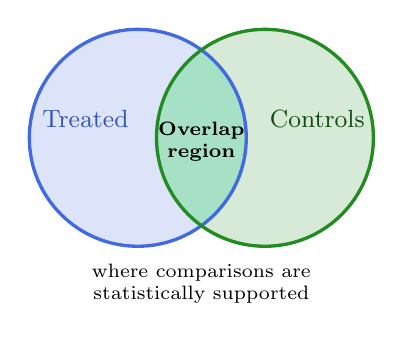
\begin{tikzpicture}[scale=0.95, every node/.style={font=\small}]
                \def\r{1.45}
                \fill[RoyalBlue!18] (-0.85,0) circle (\r);
                \fill[ForestGreen!18] (0.85,0) circle (\r);
                \begin{scope}
                    \clip (-0.85,0) circle (\r);
                    \fill[blue!35!green!35] (0.85,0) circle (\r);
                \end{scope}
                \draw[RoyalBlue, very thick] (-0.85,0) circle (\r);
                \draw[ForestGreen, very thick] (0.85,0) circle (\r);
                \node[RoyalBlue!80!black] at (-1.55,0.25) {Treated};
                \node[ForestGreen!55!black] at (1.55,0.25) {Controls};
                \node[align=center, font=\scriptsize\bfseries, text=black] at (0,-0.05) {Overlap\\region};
                \node[align=center, font=\scriptsize, text=black] at (0,-1.95) {where comparisons are\\statistically supported};
            \end{tikzpicture}
        \end{column}
    \end{columns}
\end{frame}

\begin{frame}{Strict Overlap in Observational Data}
    \begin{itemize}
       \item Strict overlap is typically guaranteed by design in many RCTs, but it is \textcolor{blue}{not automatic in observational data}
        $\Longrightarrow$ \textcolor{blue}{we restrict attention to regions with sufficient overlap}
        \bigskip

        \item This changes the welfare object from $W(h_0)$ to an overlap-restricted criterion:
            \[
               W_\alpha(h_0)
               =
               \int_\mathcal{X} \mathbbm{1}\{h_{0}(x) \geq 0\} 
               \textcolor{blue}{\mathbbm{1}\{\alpha < p_0(D =1 \mid X = x) <  1- \alpha\}}
               h_0(x)f(x)dx
            \]

        \item This also aligns with the common practice of trimming observations with extreme estimated propensity scores:
            \[
            \alpha \equiv 0.05, 0.1,\ldots
            \] 
    \end{itemize}
\end{frame}

\begin{frame}{Admissibility-Constrained Treatment-Choice Problem}
    \begin{itemize}
        \item A policymaker often faces a constrained treatment-allocation problem
        \citep*{FengHongNekipelov2026}:
            \[
            \max_{\phi \in \Phi}
            \mathbb{E}\left[
            Y_1\phi(X) + Y_0(1- \phi(X))
            \right]
            \quad
            \text{s.t.}
            \quad
            \mathbb{E}\left[
            Z_1\phi(X) + Z_0(1-\phi(X))
            \right] \leq \alpha.
            \]
            \vspace{-0.9em}
            \begin{itemize}
                \item[-] $Y_1$ and $Y_0$ are welfare outcomes with and without treatment;
                \item[-] $Z_1$ and $Z_0$ are the corresponding costs under treatment and control.
            \end{itemize}
            
        \bigskip
        \item The optimal rule treats covariate type $X=x$ when the welfare gain is large enough to justify the additional cost:
            \[
            \mathbbm{1}\left\{
            \mathbb{E}[Y_1 - Y_0 \mid X=x]
            -
            k\mathbb{E}[Z_1 - Z_0 \mid X=x]
            \geq 0
            \right\}.
            \]
            \vspace{-0.9em}
            \begin{itemize}
                \item[-] $k$ is the shadow price of the resource constraint;
                \item[-] Smaller $\alpha$ $\Rightarrow$ larger $k$; larger $\alpha$ $\Rightarrow$ smaller $k$;
                \item[-] This criterion is \textcolor{blue}{compensatory}: sufficiently large benefits can justify higher costs.
            \end{itemize}
    \end{itemize}
\end{frame}

\begin{frame}{Admissibility-Constrained Treatment-Choice Problem}
    \begin{itemize}
        \item In some settings, however, a high cost cannot be compensated by a high benefit:
            \begin{itemize}
                \item[-] Example: severe side effects, measured by
                $\mathbb{E}[Z_1-Z_0\mid X]$.
                \item[-] If the \textcolor{blue}{side effect} is sufficiently severe, the policymaker may refuse treatment regardless of the expected benefit.
            \end{itemize}
        \bigskip

        \item This corresponds to a \textcolor{blue}{checklist-style admissibility criterion}:
            \begin{itemize}
                \item[-] Treatment is considered only for individuals who pass the safety screen;
                \item[-] No health benefit can compensate for failing the safety screen;
                \item[-] This echoes the Hippocratic principle: \textcolor{blue}{``First, do no harm.''}
            \end{itemize}
    \end{itemize}
\end{frame}

\begin{frame}{Admissibility-Constrained Treatment-Choice Problem}
    \begin{itemize}
        \item The policymaker's problem becomes:
            \[
            \max_{\phi \in \Phi}
            \mathbb{E}\left[
            Y_1\phi(X)+Y_0(1-\phi(X))
            \right]
            \]
            \[
            \text{s.t.}\quad
            \phi(x)
            \leq
            \mathbbm{1}\left\{
            \mathbb{E}[Z_1-Z_0 \mid X=x]\leq \bar z
            \right\},
            \quad \forall x\in\mathcal{X}.
            \]

        \item The optimal welfare under this treatment rule is:
            \[
            \int_\mathcal{X}
            \mathbbm{1}\left\{\mathbb{E}[Y_1-Y_0\mid X=x]\geq 0\right\}
            \textcolor{blue}{
            \mathbbm{1}\left\{\mathbb{E}[Z_1-Z_0\mid X=x]\leq \bar z\right\}
            }
            \mathbb{E}[Y_1-Y_0\mid X=x]
            f(x)dx.
            \]
    \end{itemize}
\end{frame}

\begin{frame}{Descriptive Statistics}
    \begin{itemize}
        \item To better understand the consequences of implementing an optimal policy, policymakers may want summary statistics beyond the welfare value:
            \begin{itemize}
                \item[-] average characteristics of those assigned to treatment;
                \item[-] average cost of the policy;
                \item[-] population share assigned to treatment.
            \end{itemize}

        \bigskip
        \item With richer data and more structured causal models, these summary statistics can involve additional causal objects.

        \bigskip
        \item This naturally leads to double-threshold functionals: one threshold defines the treatment rule, while the other describes a policy-relevant feature of the population.
    \end{itemize}
\end{frame}

\begin{frame}{Descriptive Statistics: Surrogate Outcomes}
\bigskip
\centering
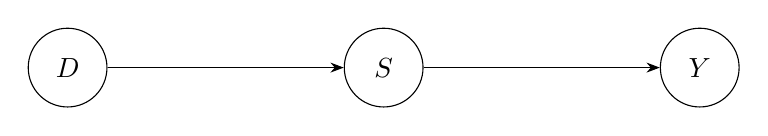
\begin{tikzpicture}[
    >=Stealth,
    node distance=3cm,
    every node/.style={draw, circle, minimum size=1.0cm, align=center}
]
    \node (D) {$D$};
    \node[right=of D] (S) {$S$};
    \node[right=of S] (Y) {$Y$};

    \draw[->] (D) -- (S);
    \draw[->] (S) -- (Y);
\end{tikzpicture}
\bigskip
\begin{itemize}
    \item \textcolor{blue}{Surrogate index setting} \citep*{AtheyChettyImbensKang2025}:
    \begin{itemize}
        \item[-] experimental data identify the effect of $D$ on short-term surrogates $S$;
        \item[-] auxiliary observational data link surrogates $S$ to long-term outcome $Y$.
    \end{itemize}

    \item A policymaker may assign treatment based on short-term surrogate gains, but still want to know whether long-run gains are positive.

    \item A useful summary statistic is the population share treated by the surrogate-based rule whose long-run treatment effect is also positive:
\end{itemize}

    \[
    \int_\mathcal{X} \mathbbm{1}\{\mathbb{E}[S(1) - S(0) \mid X=x] \geq 0\}\textcolor{blue}{\mathbbm{1}\{\mathbb{E}[Y(1) - Y(0) \mid X=x] \geq 0\}}f(x)dx
    \]
\end{frame}

\begin{frame}{Descriptive Statistics: Mediation}
\centering
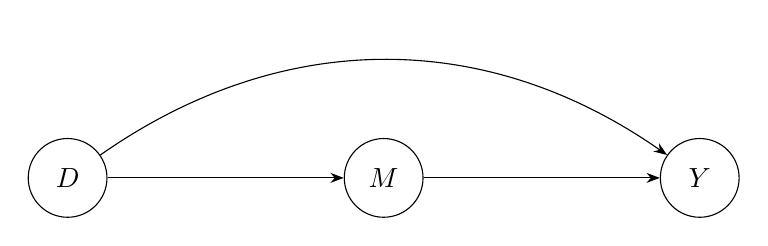
\begin{tikzpicture}[
    >=Stealth,
    node distance=3cm,
    every node/.style={draw, circle, minimum size=1.0cm, align=center}
]
    \node (D) {$D$};
    \node[right=of D] (M) {$M$};
    \node[right=of M] (Y) {$Y$};

    \draw[->] (D) -- (M);
    \draw[->] (M) -- (Y);
    \draw[->] (D) to[bend left=35] (Y);
\end{tikzpicture}

\begin{itemize}
    \item \textcolor{blue}{Causal mediation analysis} \citep*{ImaiKeeleTingley2010} studies how treatment effects operate through intermediate mechanisms.

    \item Example: $D$ is access to cognitive behavioral therapy, $M$ is household support, and $Y$ is financial empowerment.

    \item A useful summary statistic is the population share optimally treated for $Y$ whose mediated contribution through $M$ is positive:
\end{itemize}

    \[
    \int_\mathcal{X} \mathbbm{1}\{\mathbb{E}[Y(1) - Y(0) \mid X=x] \geq 0\}\textcolor{blue}{\mathbbm{1}\{\mathbb{E}\left[Y(1,M(1))-Y(1,M(0))\mid X=x\right]\geq 0\}}f(x)dx
    \]
\end{frame}




\begin{frame}{Dynamic Treatment Regime}
    \begin{itemize}
        \item Consider the setting in \citet*{chen2023inference} and \citet*{whitehouse2026inference}: We assume access to i.i.d. samples $Z \sim P_Z$ of the form $Z = (X_1,A_1,X_2,A_2, Y)$ that are generated according to the following structural equation model.
            \begin{align*}
                Y &= f_Y(A_2, X_2, \xi_Y)\\
                A_2 &= f_{A_2}(X_2, \xi_{A_2})\\
                X_2 &= f_{X_2}(A_2, X_1, \xi_{X_2})\\
                A_1 &= f_{A_1}(X_1, \xi_{A_1})\\
                X_1 &= f_{X_1}(\xi_{X_1})
            \end{align*}
    \end{itemize}
    \centering
    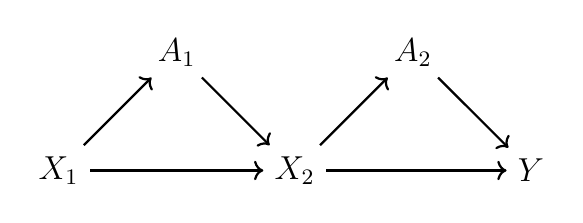
\begin{tikzpicture}\large
        \node (X1) at (0,0) {$X_1$};
        \node (A1) at (1.5,1.5) {$A_1$};
        \node (X2) at (3,0) {$X_2$};
        \node (A2) at (4.5,1.5) {$A_2$};
        \node (Y)  at (6,0) {$Y$};
    
        \draw[thick,->] (X1) -- (A1);
        \draw[thick,->] (X1) -- (X2);
        \draw[thick,->] (A1) -- (X2);
        \draw[thick,->] (X2) -- (A2);
        \draw[thick,->] (X2) -- (Y);
        \draw[thick,->] (A2) -- (Y);
    \end{tikzpicture}
\end{frame}

\begin{frame}{Dynamic Treatment Regime}
    \begin{itemize}
        \item Dynamic treatment regime:
            \[
            \pi_1:\mathcal{X}_1 \rightarrow \{0,1\}
            \]
            \[
            \pi_2:\mathcal{X}_2 \rightarrow \{0,1\}
            \]
    
        \item Potential outcome under dynamic treatment regime
            \[
                Y := Y^{(A_1, A_2)}
            \]
            \[
                Y^{(\tau_1,\pi_2)}
                :=
                \sum_{\tau_2\in\{0,1\}}
                \mathbbm 1\left\{\pi_2\left(X_2^{(\tau_1)}\right)=\tau_2\right\}
                Y^{(\tau_1,\tau_2)}.
            \]
            \[
                Y^{(\pi_1,\pi_2)}
                :=
                \sum_{\tau_1\in\{0,1\}}
                \mathbbm 1\{\pi_1(X_1)=\tau_1\}
                Y^{(\tau_1,\pi_2)}.
            \]
    \end{itemize}
\end{frame}

\begin{frame}{Dynamic Treatment Regime}
    \begin{itemize}
        \item Assume sequential independence and perform backward induction to solve for the optimal dynamic treatment regime
            \[
            Y^{(T_1, \pi_2 )} \perp A_2 \mid X_2, \quad Y^{(\pi_1, \pi_2)} \perp A_1 \mid X_1
            \]

        \item Optimal treatment in period 2:
            \[
                \pi_2^*(x_2) \in \operatorname*{arg\,max}_{a\in\{0,1\}} \mu_{a}(x_2), \quad \mu_a(x) = \mathbb{E}[Y\mid X_2 = x_2, A_2 = a]
            \]
        \item Optimal treatment in period 1:
            \[
                \pi_1^*(s) \in \operatorname*{arg\,max}_{\tau_1\in\{0,1\}} \mathbb E[V_2(X_2)\mid X_1=x_1,A_1=\tau_1], \quad V_2(x_2) := \max\{\mu_0(x_2),\mu_1(x_2)\}
            \]
    \end{itemize}
\end{frame}

\begin{frame}{Dynamic Treatment Regime}
    \begin{itemize}
        \item \textcolor{blue}{Total optimal policy value:}
            \begin{align*}
                &\quad V^*
                = \mathbb{E}\left[Y^{(\pi^*_1, \pi^*_2)}\right]\\
                &= \mathbb E\!\left[
                Y^{(0,0)}
                \mathbbm 1\{\pi_1^*(X_1)=0,\pi_2^*(X^{(0)}_2)=0\}
                \right]+
                \mathbb E\!\left[
                Y^{(1,0)}
                \mathbbm 1\{\pi_1^*(X_1)=1,\pi_2^*(X^{(1)}_2)=0\}
                \right] \\
                &\quad+
                \mathbb E\!\left[
                Y^{(0,1)}
                \mathbbm 1\{\pi_1^*(X_1)=0,\pi_2^*(X^{(0)}_2)=1\}
                \right] +
                \mathbb E\!\left[
                Y^{(1,1)}
                \mathbbm 1\{\pi_1^*(X_1)=1,\pi_2^*(X^{(1)}_2)=1\}
                \right]
            \end{align*}

        \item Using a smoothing technique, \citet*{whitehouse2026inference} shows $V^*$ is parametrically estimable and constructs corresponding CIs.

        \item However, it might be interesting to draw inference on \textcolor{blue}{welfare coming from each treatment path}, say
            \[
            V^*_{11} = \mathbb E\!\left[
                Y^{(1,1)}
                \mathbbm 1\{\pi_1^*(X_1)=1,\pi_2^*(X^{(1)}_2)=1\}
                \right]
            \]

    \end{itemize}
\end{frame}

\begin{frame}{Dynamic Treatment Regime}
    \begin{align*}
        V^*_{11} &= \mathbb E\!\left[
                Y^{(1,1)}
                \mathbbm 1\left\{\pi_1^*(X_1)=1,\pi_2^*(X^{(1)}_2)=1\right\}
                \right]\\
        &=
        \int_{\mathcal X_2}
        \int_{\mathcal X_1}
        \textcolor{blue}{\mathbbm 1\{\delta(x_2)\geq 0\}
        \mathbbm 1\{\kappa(x_1)\geq 0\}}
        \mu_1(x_2)p_1(x_2\mid x_1)m(x_1)\,\mathrm dx_1\,\mathrm dx_2
    \end{align*}
    with 
    \[
    \delta(x_2) = \mu_1(x_2) - \mu_0(x_2)
    \]
    \[
    \kappa(x_1) = \mathbb{E}[V_2(X_2) \mid X_1 = x_1, A_1 = 1] - \mathbb{E}[V_2(X_2) \mid X_1 = x_1, A_1 = 0]
    \]
    \begin{itemize}
        \item The boundary $\{\kappa(x_1) = 0\}$ is smooth because $\max$ is smoothed out by conditional expectation
    \end{itemize}
\end{frame}

\begin{frame}{Dynamic Treatment Regime}
    \begin{itemize}
        \item Assuming $p_1(x_2 \mid x_1) = \Pr(X_2 = x_2 \mid X_1 =x_1, A_1 = 1)$ is known, I have shown that $V^*_{11}$ is irregular

        \bigskip

        \item In particular, $DV^*_{11}[\dot{\mu}_0, \dot{\mu}_1] = \text{standard linear functional} + B_{11}^{M_1} + B_{11}^{M_2}$

        \bigskip

        \item Why is $V^*$ regular? \textcolor{blue}{This is because boundary terms cancel out.}
            \[
            B_{11}^{M_1} +  B_{10}^{M_1} + B_{01}^{M_1} + B_{00}^{M_1} = 0
            \]
            \[
            B_{11}^{M_2} +  B_{10}^{M_2} + B_{01}^{M_2} + B_{00}^{M_2} = 0            
            \]
    \end{itemize}
\end{frame}

\begin{frame}{Conclusion}
    In this paper,
    \begin{itemize}
        \item I want to study inference on optimal policy values or related statistics in settings existing work could not handle;
        \bigskip
        \item I would like to extend the advanced machinery in \citet*{chen2025inference} to these new settings;
        \bigskip
        \item I would hope to sell this idea to practitioners.
    \end{itemize}
\end{frame}



%------------------------------------------------

\begin{frame}{References}
    \footnotesize
    \bibliography{reference}
    \bibliographystyle{plainnat}
\end{frame}

%------------------------------------------------

\begin{frame}
    \Huge{\centerline{\textbf{The End}}}
\end{frame}

%----------------------------------------------------------------------------------------

\end{document}
